\subsection{Actuator scale attack}
This attack is carried out adding two extra FMUs between the \code{controller}
and the \code{plant} FMUs, one for each output of the \code{controller}.

This attack can be performed in two different ways:
\begin{enumerate}
	\item Interval Mode: In this mode the attack is performed once, for an
		interval of time defined by the attacker, starting from an
		instant chosen from the attacker.
	\item Cyclic Mode: The attack is performed periodically.
\end{enumerate}

The attacker can choose some parameters:
\begin{itemize}
	\item \code{Real attack\_time}: The time at which the attack starts.
	\item \code{Real attack\_duration}: The duration of the attack.
	\item \code{Real attack\_value}: The speed change coefficient.
	\item \code{Bool cyclic}: If \code{true} the attack is performed
		periodically.
\end{itemize}

The objective of the attack is to set the values for the actuators, contained in
the \code{plant} component, so that the robot will go at a different speed from
the right one: from the first half of \code{attack\_duration} the speed is
multiplied by \code{attack\_value}; into the second half of
\code{attack\_duration} the speed is divided by \code{attack\_value}.

\lstinputlisting[language=C, label={lst:scale_attack},
caption={Attack fmu algorithm.}]{actuator_scale_attack_fmu.c}

\begin{figure}[htb]
	\centering
	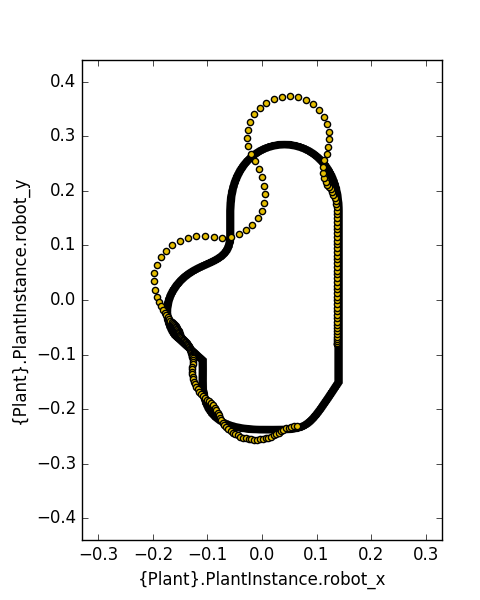
\includegraphics[width=0.5\textwidth]{actuator-scale-attack}
	\caption{Line follower robot path when
	attacked}\label{fig:actuatorscaleresult}
\end{figure}

In \figref{fig:actuatorscaleresult} we can see the result of the attack: in the
first part the robot's curves were very distant from the correct path; instead
in the second part the path is followed with more precision.
